
\subsection{Usage of AI}

OpenAI’s free LLM, ChatGPT-4o, was used to improve the grammar and wording in this work and to document the code. It also assisted in understanding the implementation of SWAG as described by \citet{maddox2019swag} (\url{https://github.com/wjmaddox/swa_gaussian/}). The tool was used to aid editorial refinements and technical understanding, not to generate original research content.


\subsection{Additional plots}

\paragraph{Tuned NN on synthetic regression and classification}
This appendix presents uncertainty estimates from the same model architectures used in Section
\ref{exp:synthetic}, now with optimized hyperparameters. Figures \ref{fig:regression_tuned} and
\ref{fig:classification_tuned} show uncertainty visualizations comparable to their non-tuned counterparts
in Figures \ref{fig:regression} and \ref{fig:classification}.

In the regression task (Figure \ref{fig:regression_tuned}), both methods exhibit visibly reduced
uncertainty compared to non-tuned results, evidenced by tighter confidence intervals throughout the domain.
For classification (Figure \ref{fig:classification_tuned}), SWAG shows substantially thinner uncertainty
estimates across the input space. MC-Dropout, however, maintains nearly identical uncertainty patterns to
its non-tuned version, with only subtle adjustments to the decision boundary attributable to improved model
performance rather than changes in uncertainty quantification behavior.

\FloatBarrier

\begin{figure}[ht]
  \centering
  \begin{subfigure}{0.8\textwidth}
    \centering
    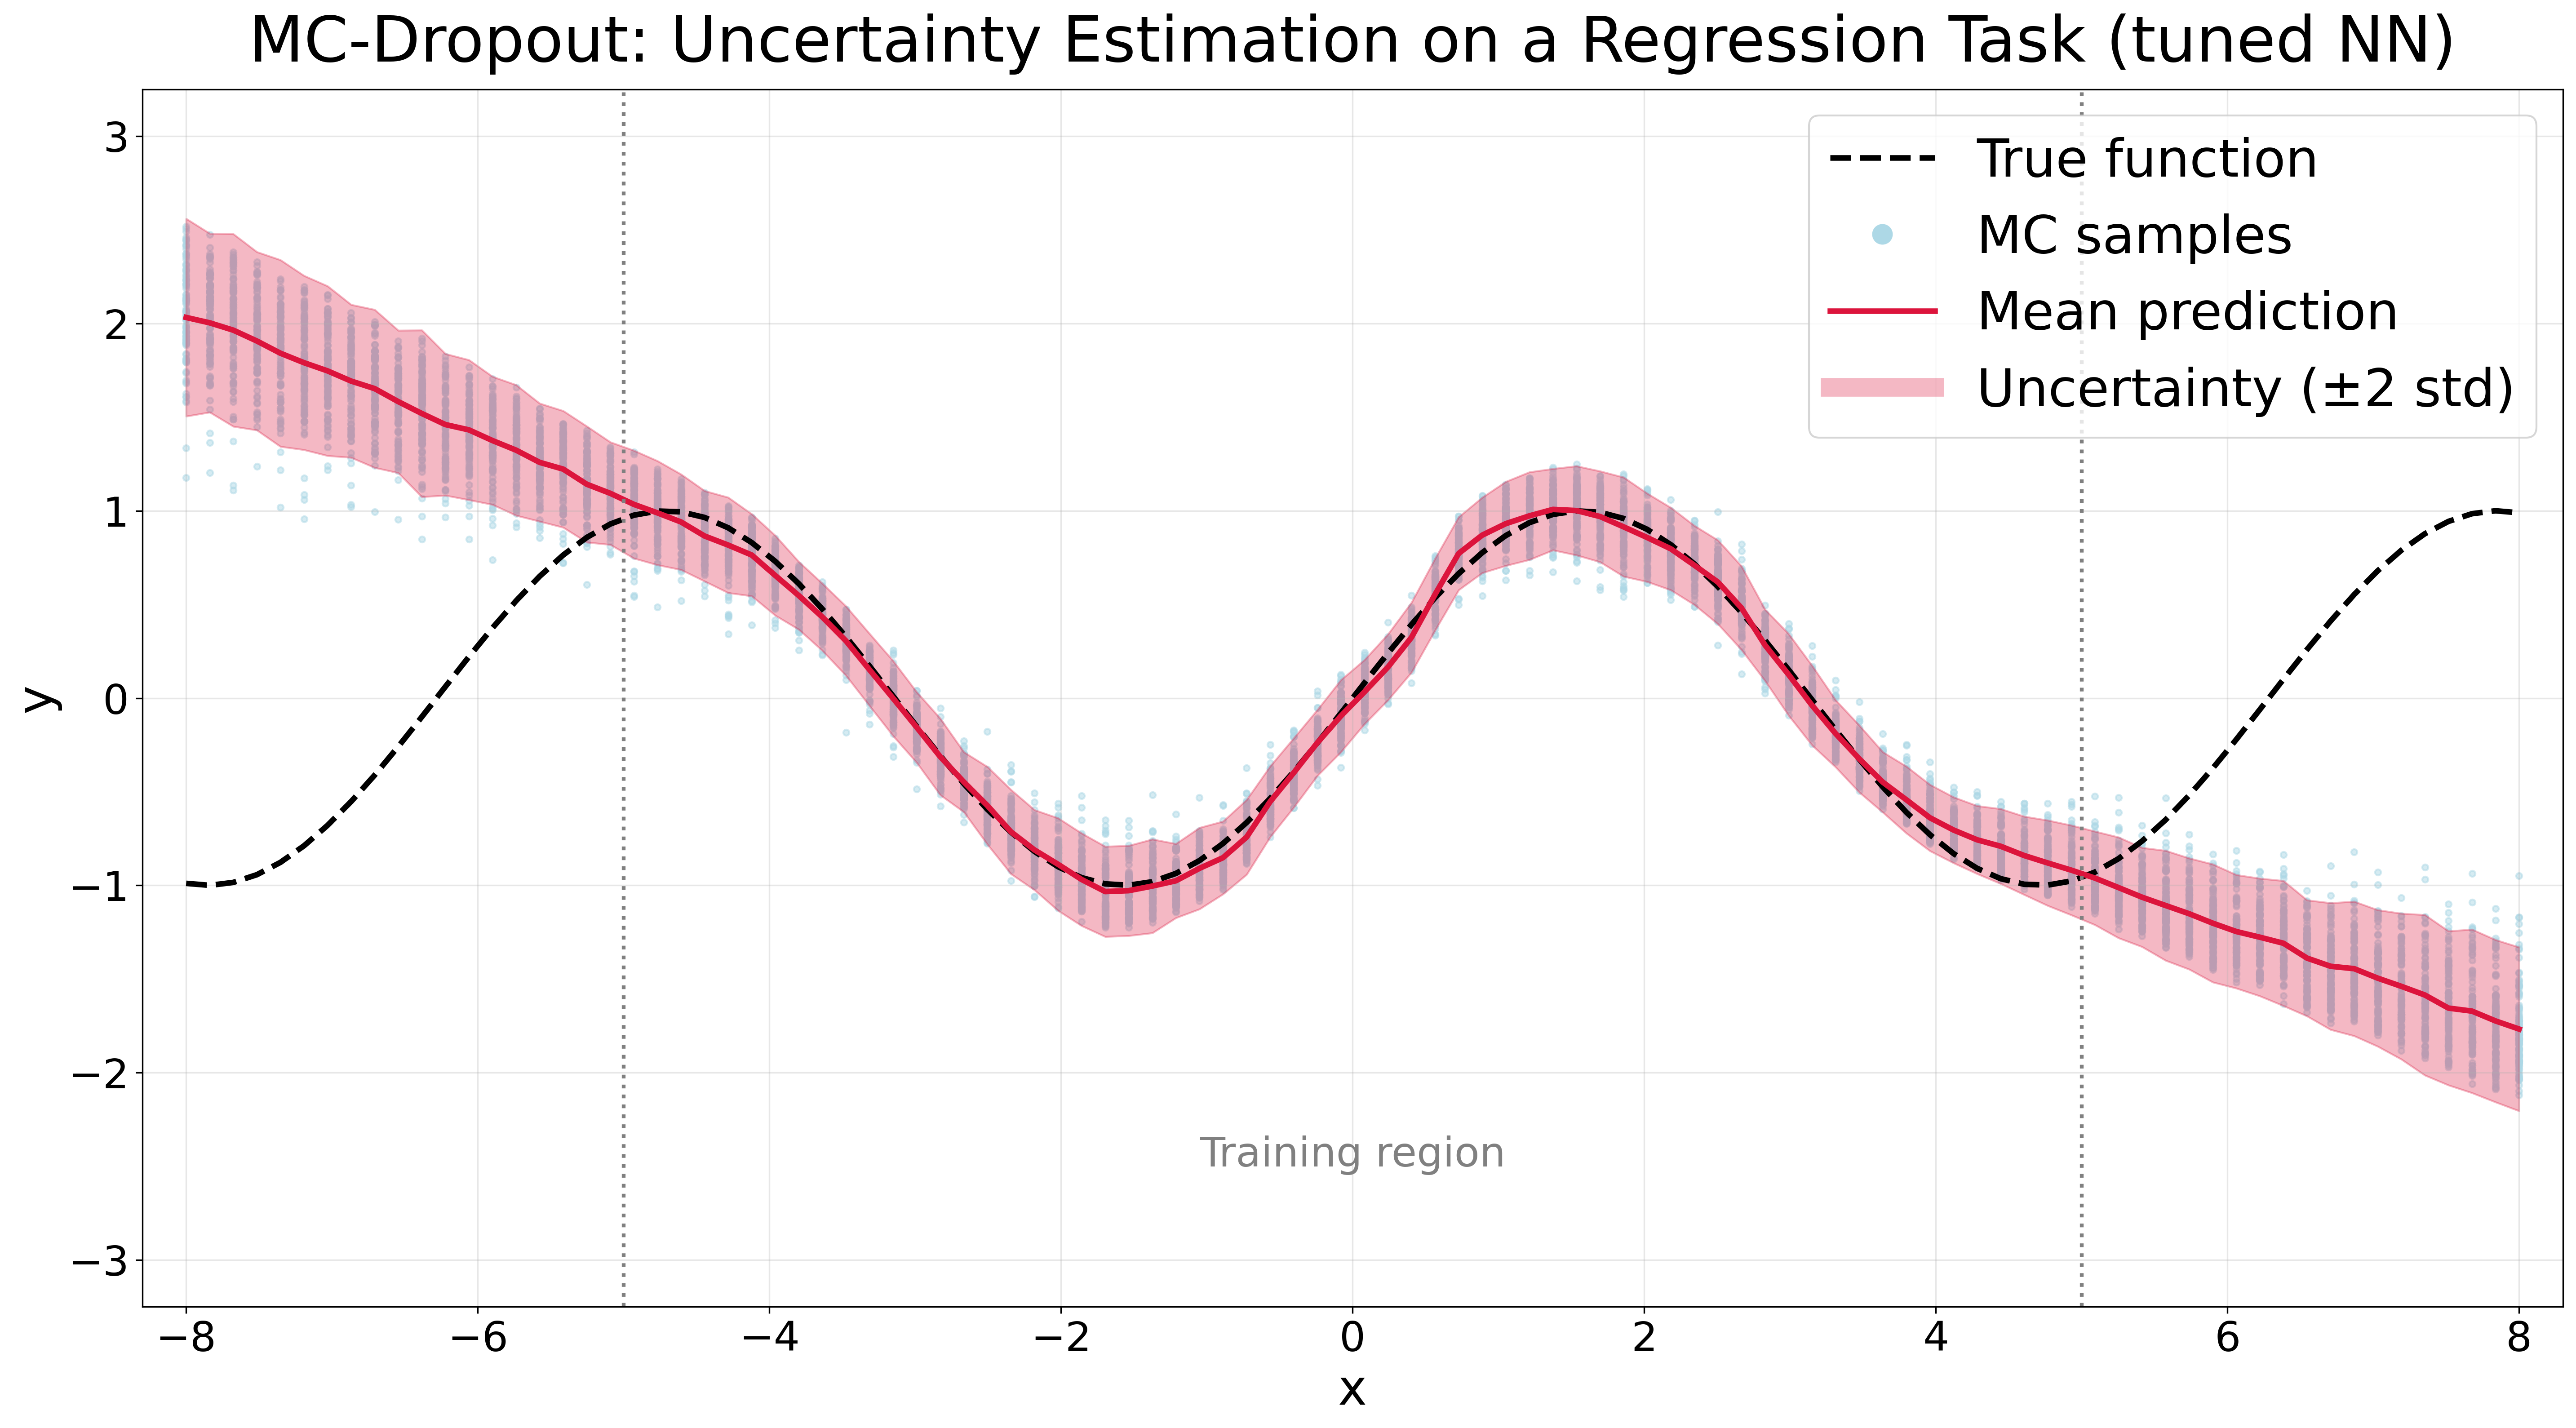
\includegraphics[width=\textwidth]{plots/mcd_reg_tuned.png}
  \end{subfigure}
  
  \vspace{0.3cm}
  \begin{subfigure}{0.8\textwidth}
    \centering
    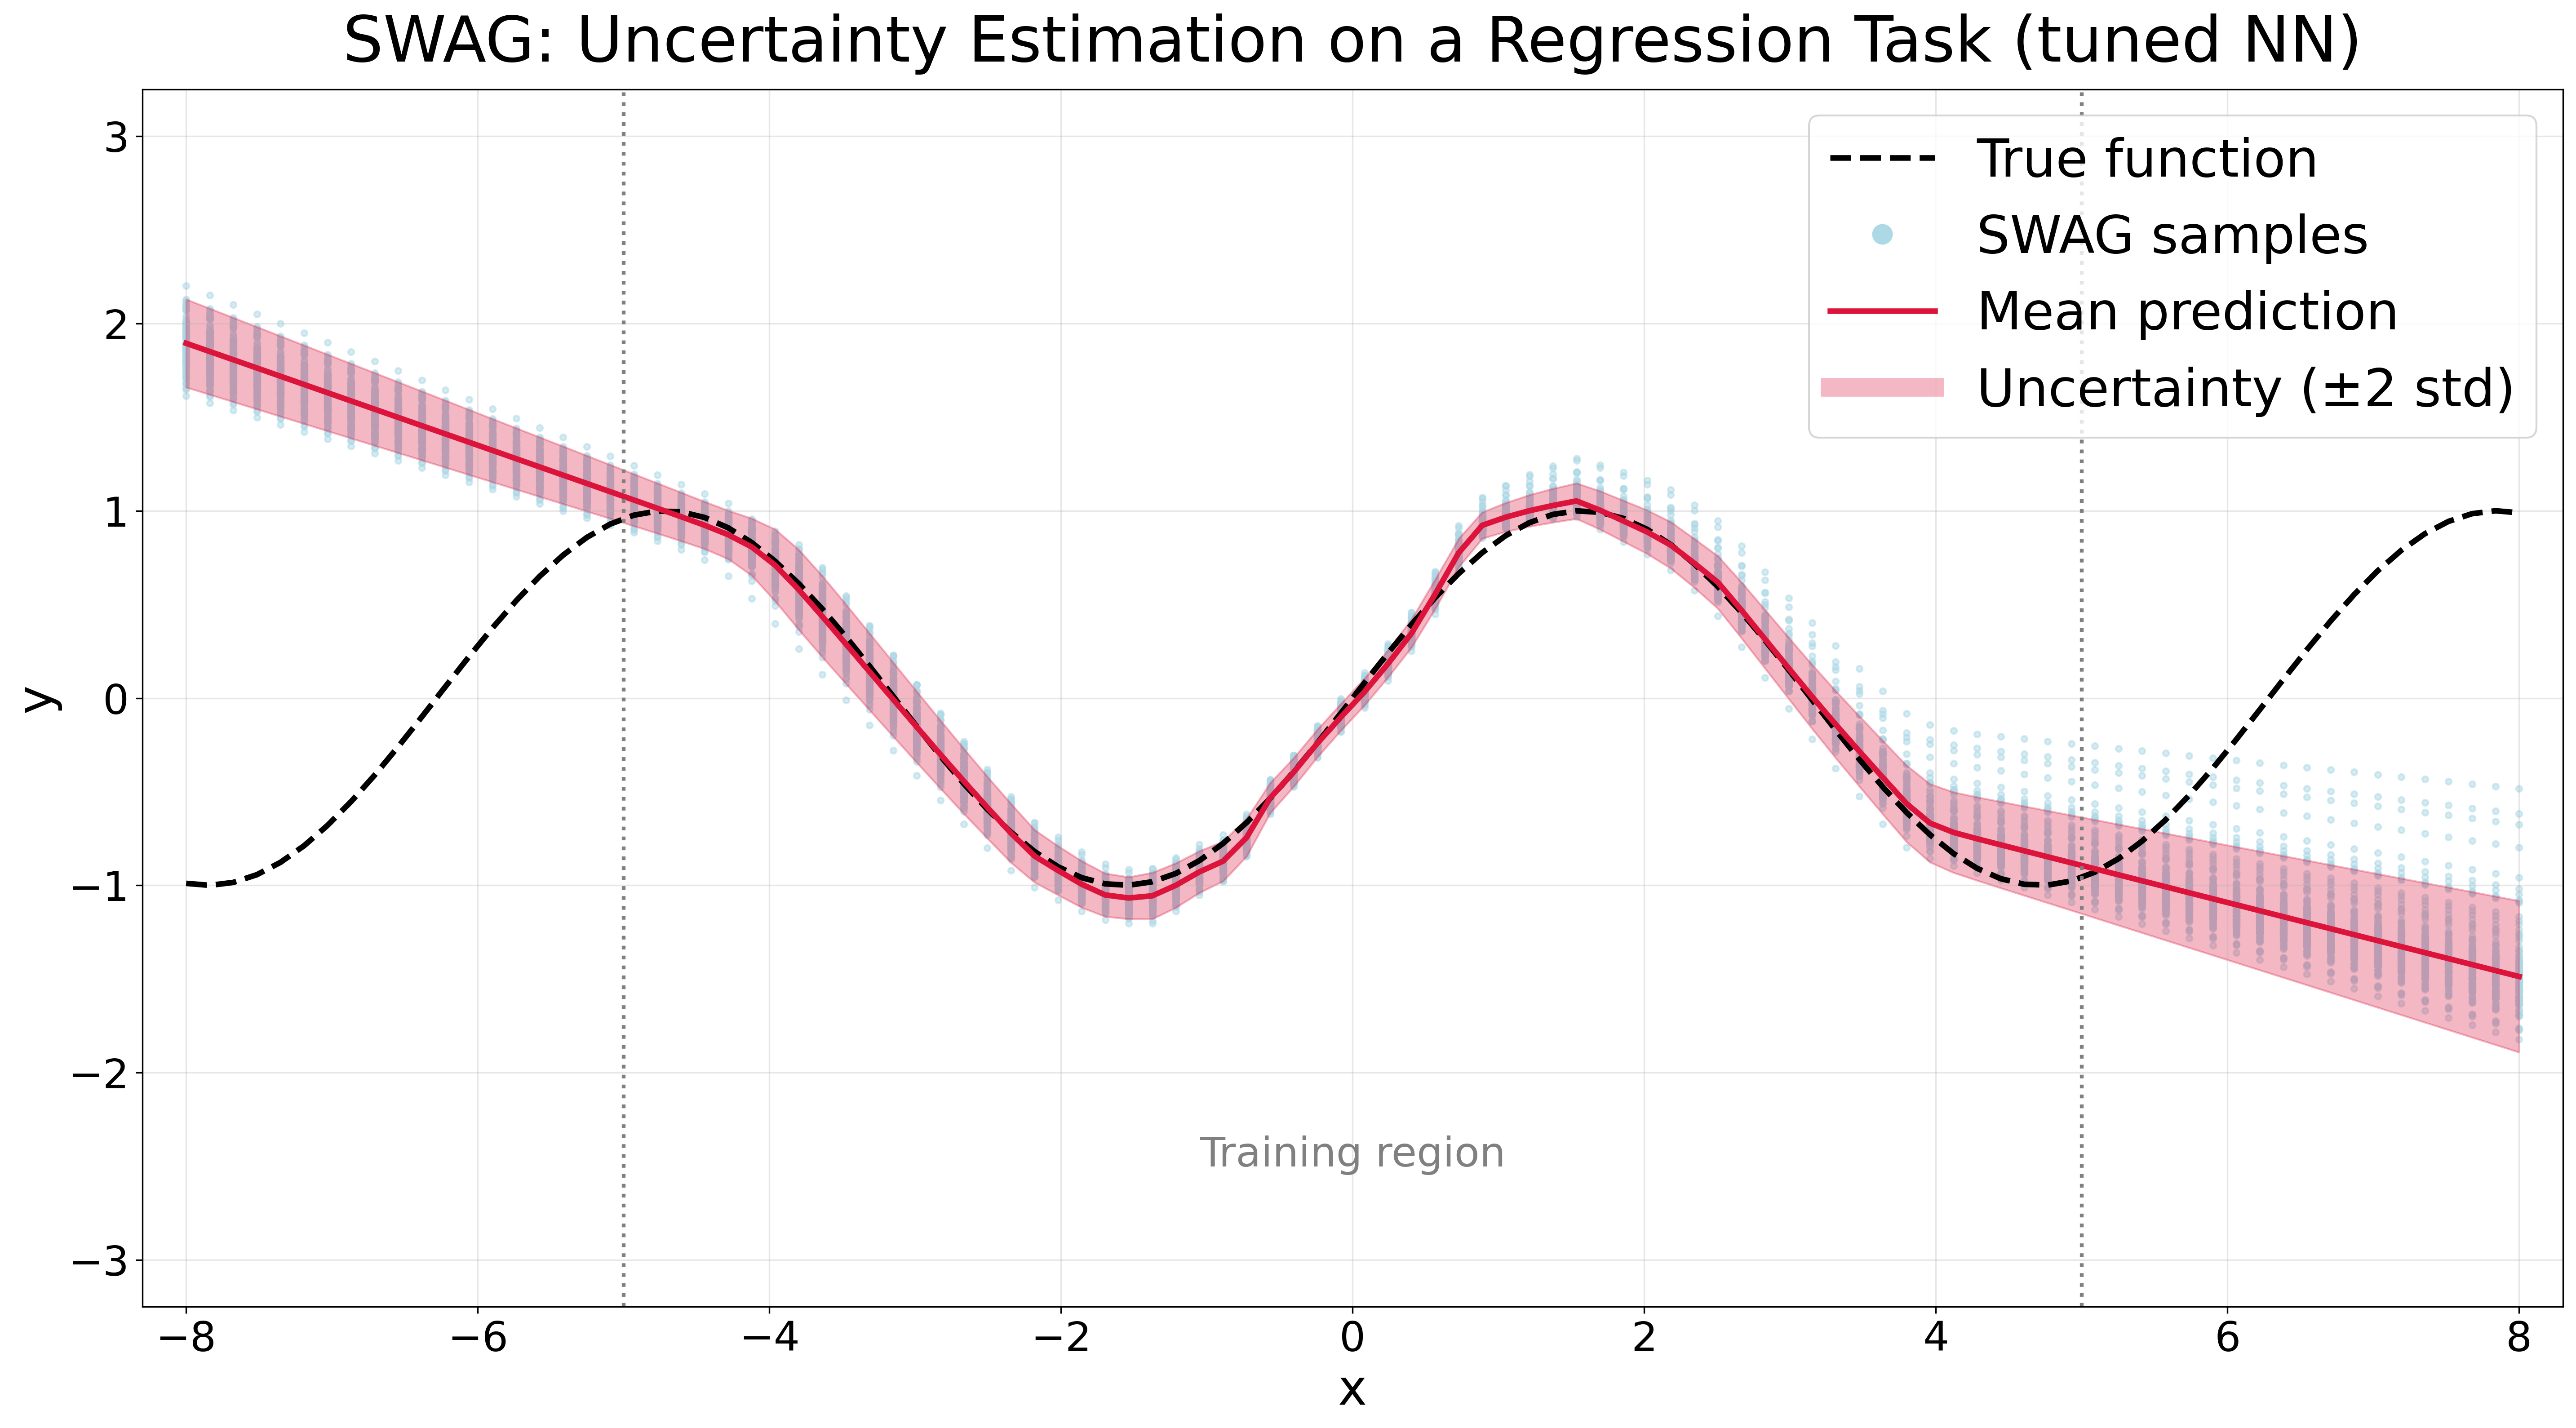
\includegraphics[width=\textwidth]{plots/swag_reg_tuned.png}
  \end{subfigure}
  \caption{Regression uncertainty estimation of a tuned Neural Network: MC-Dropout (top) and SWAG (bottom). Training domain ($|x| \leq 5$) marked by dashed lines.}
  \label{fig:regression_tuned}
\end{figure}

\begin{figure}[ht]
  \centering
  \begin{subfigure}{0.8\textwidth}
    \centering
    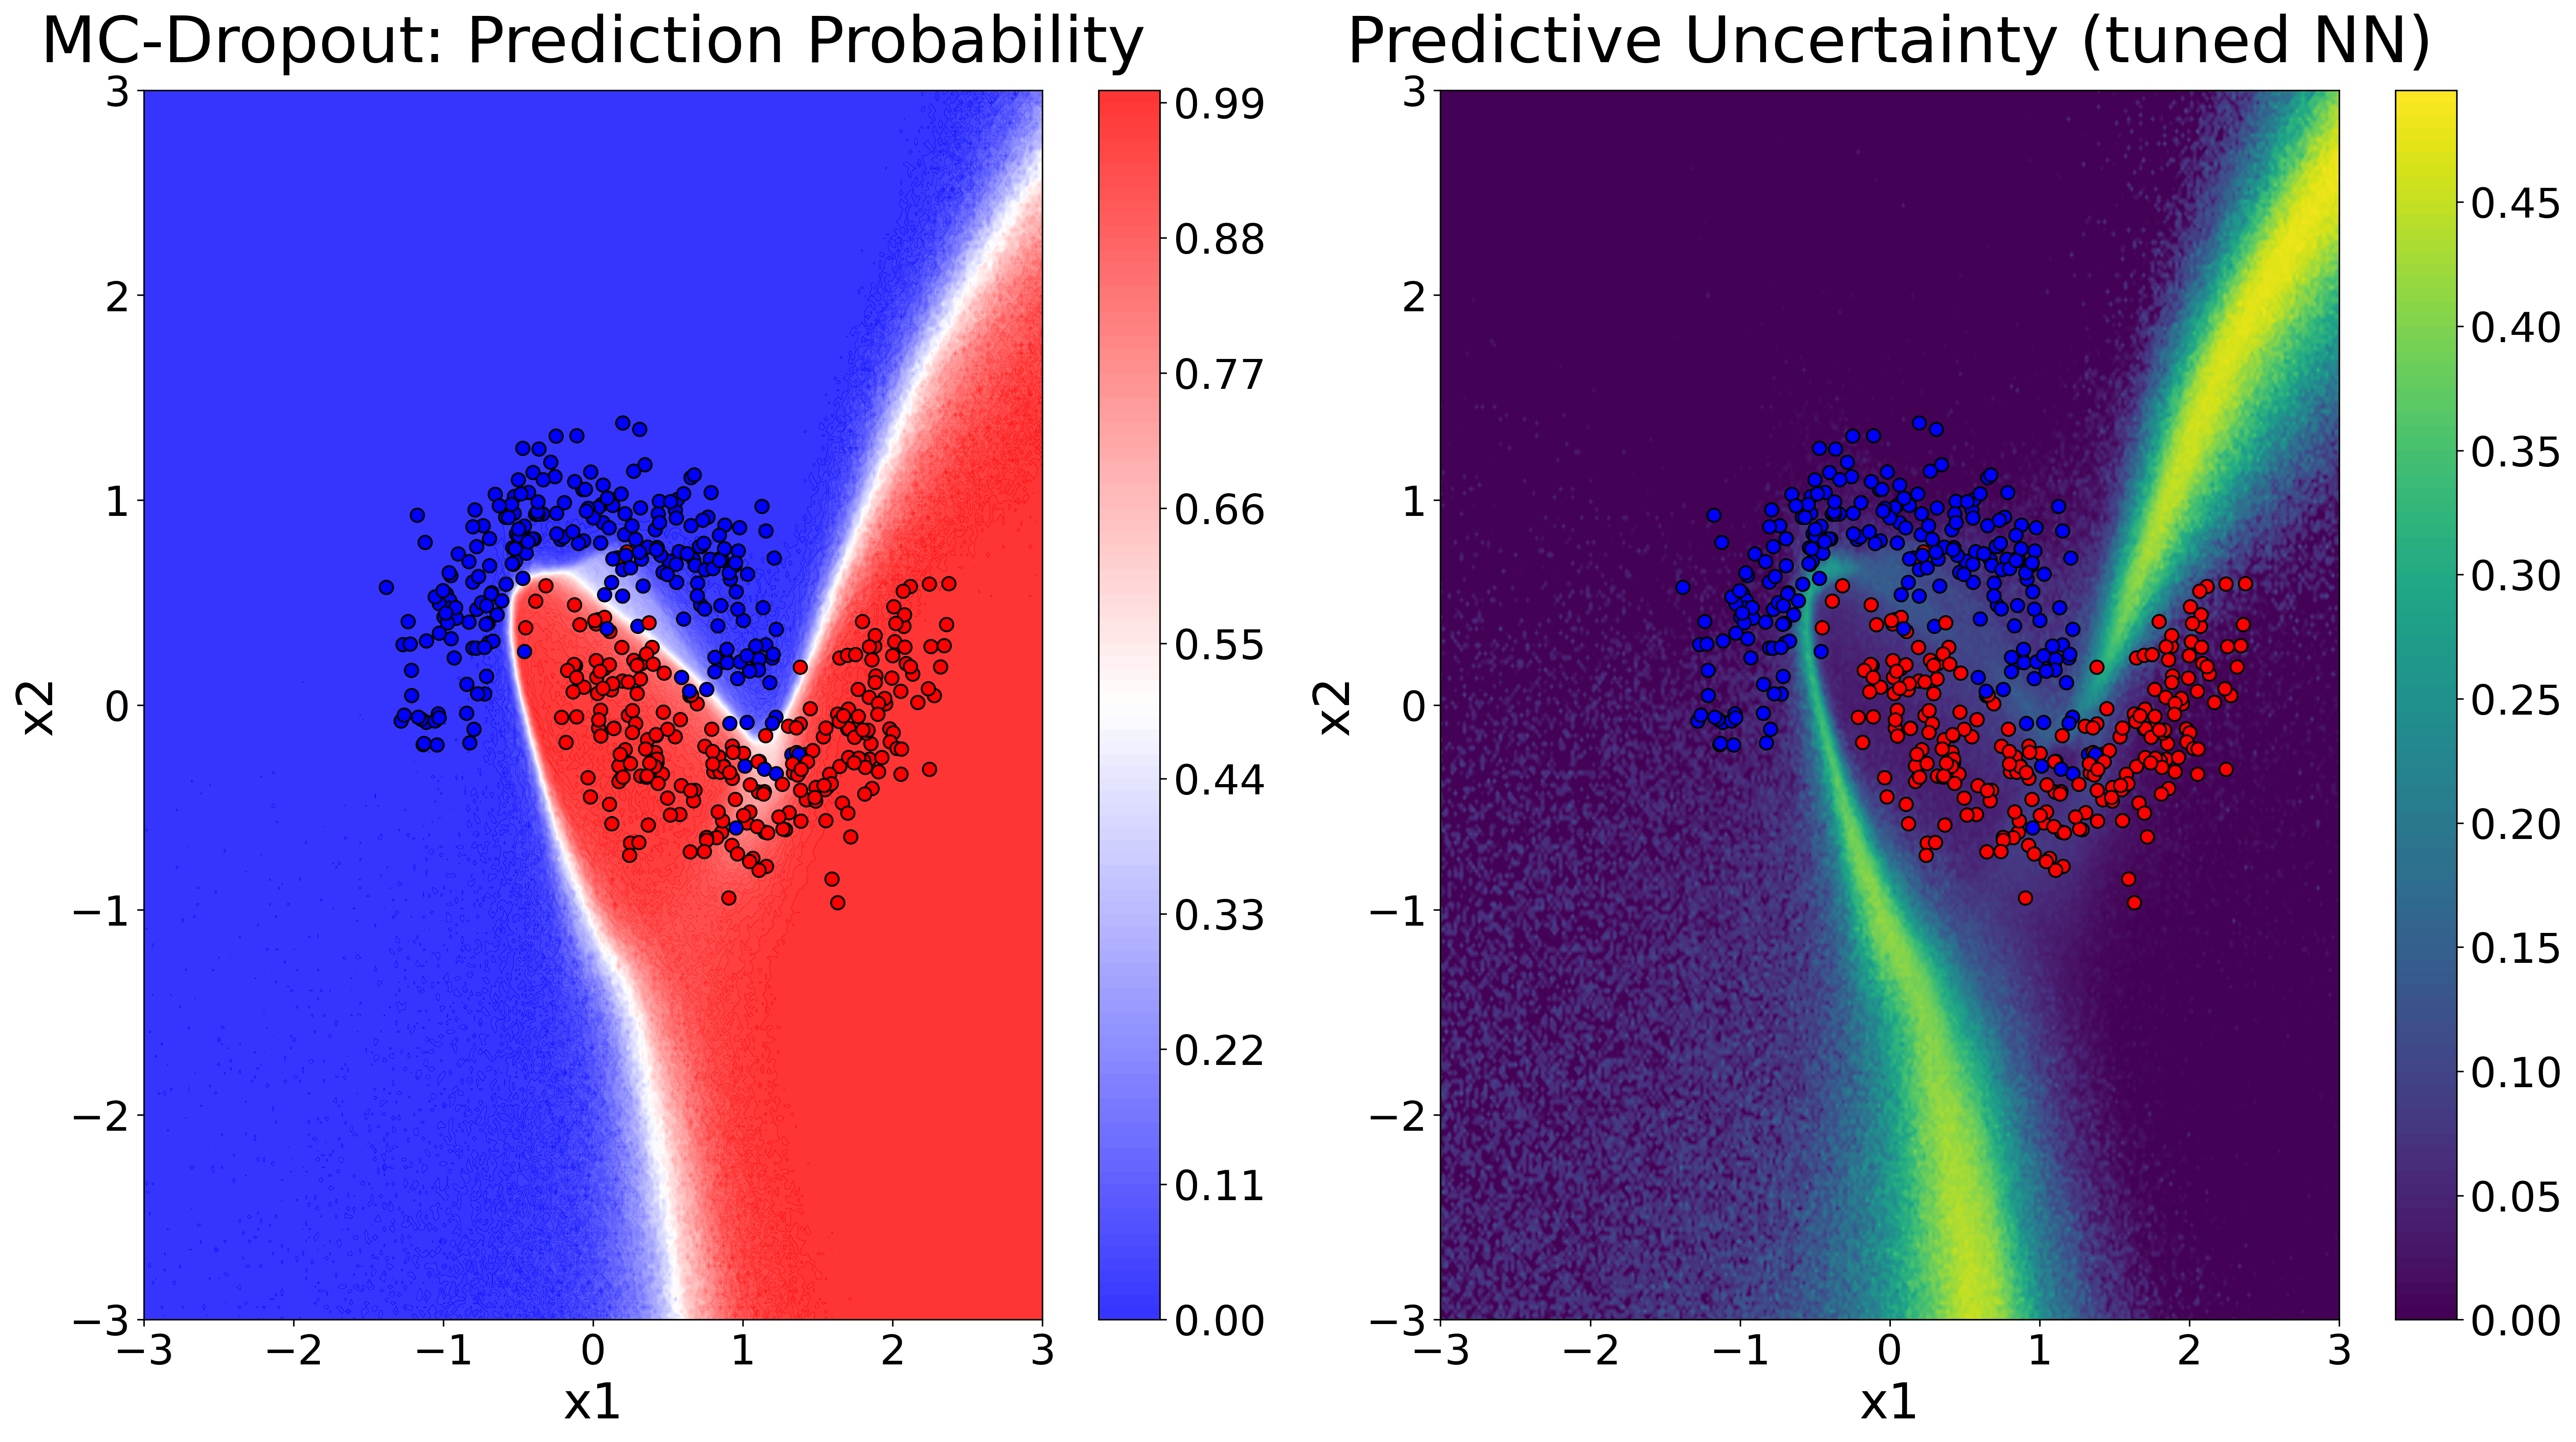
\includegraphics[width=\textwidth]{plots/mcd_cla_tuned.png}
  \end{subfigure}
  
  \vspace{0.3cm}
  \begin{subfigure}{0.8\textwidth}
    \centering
    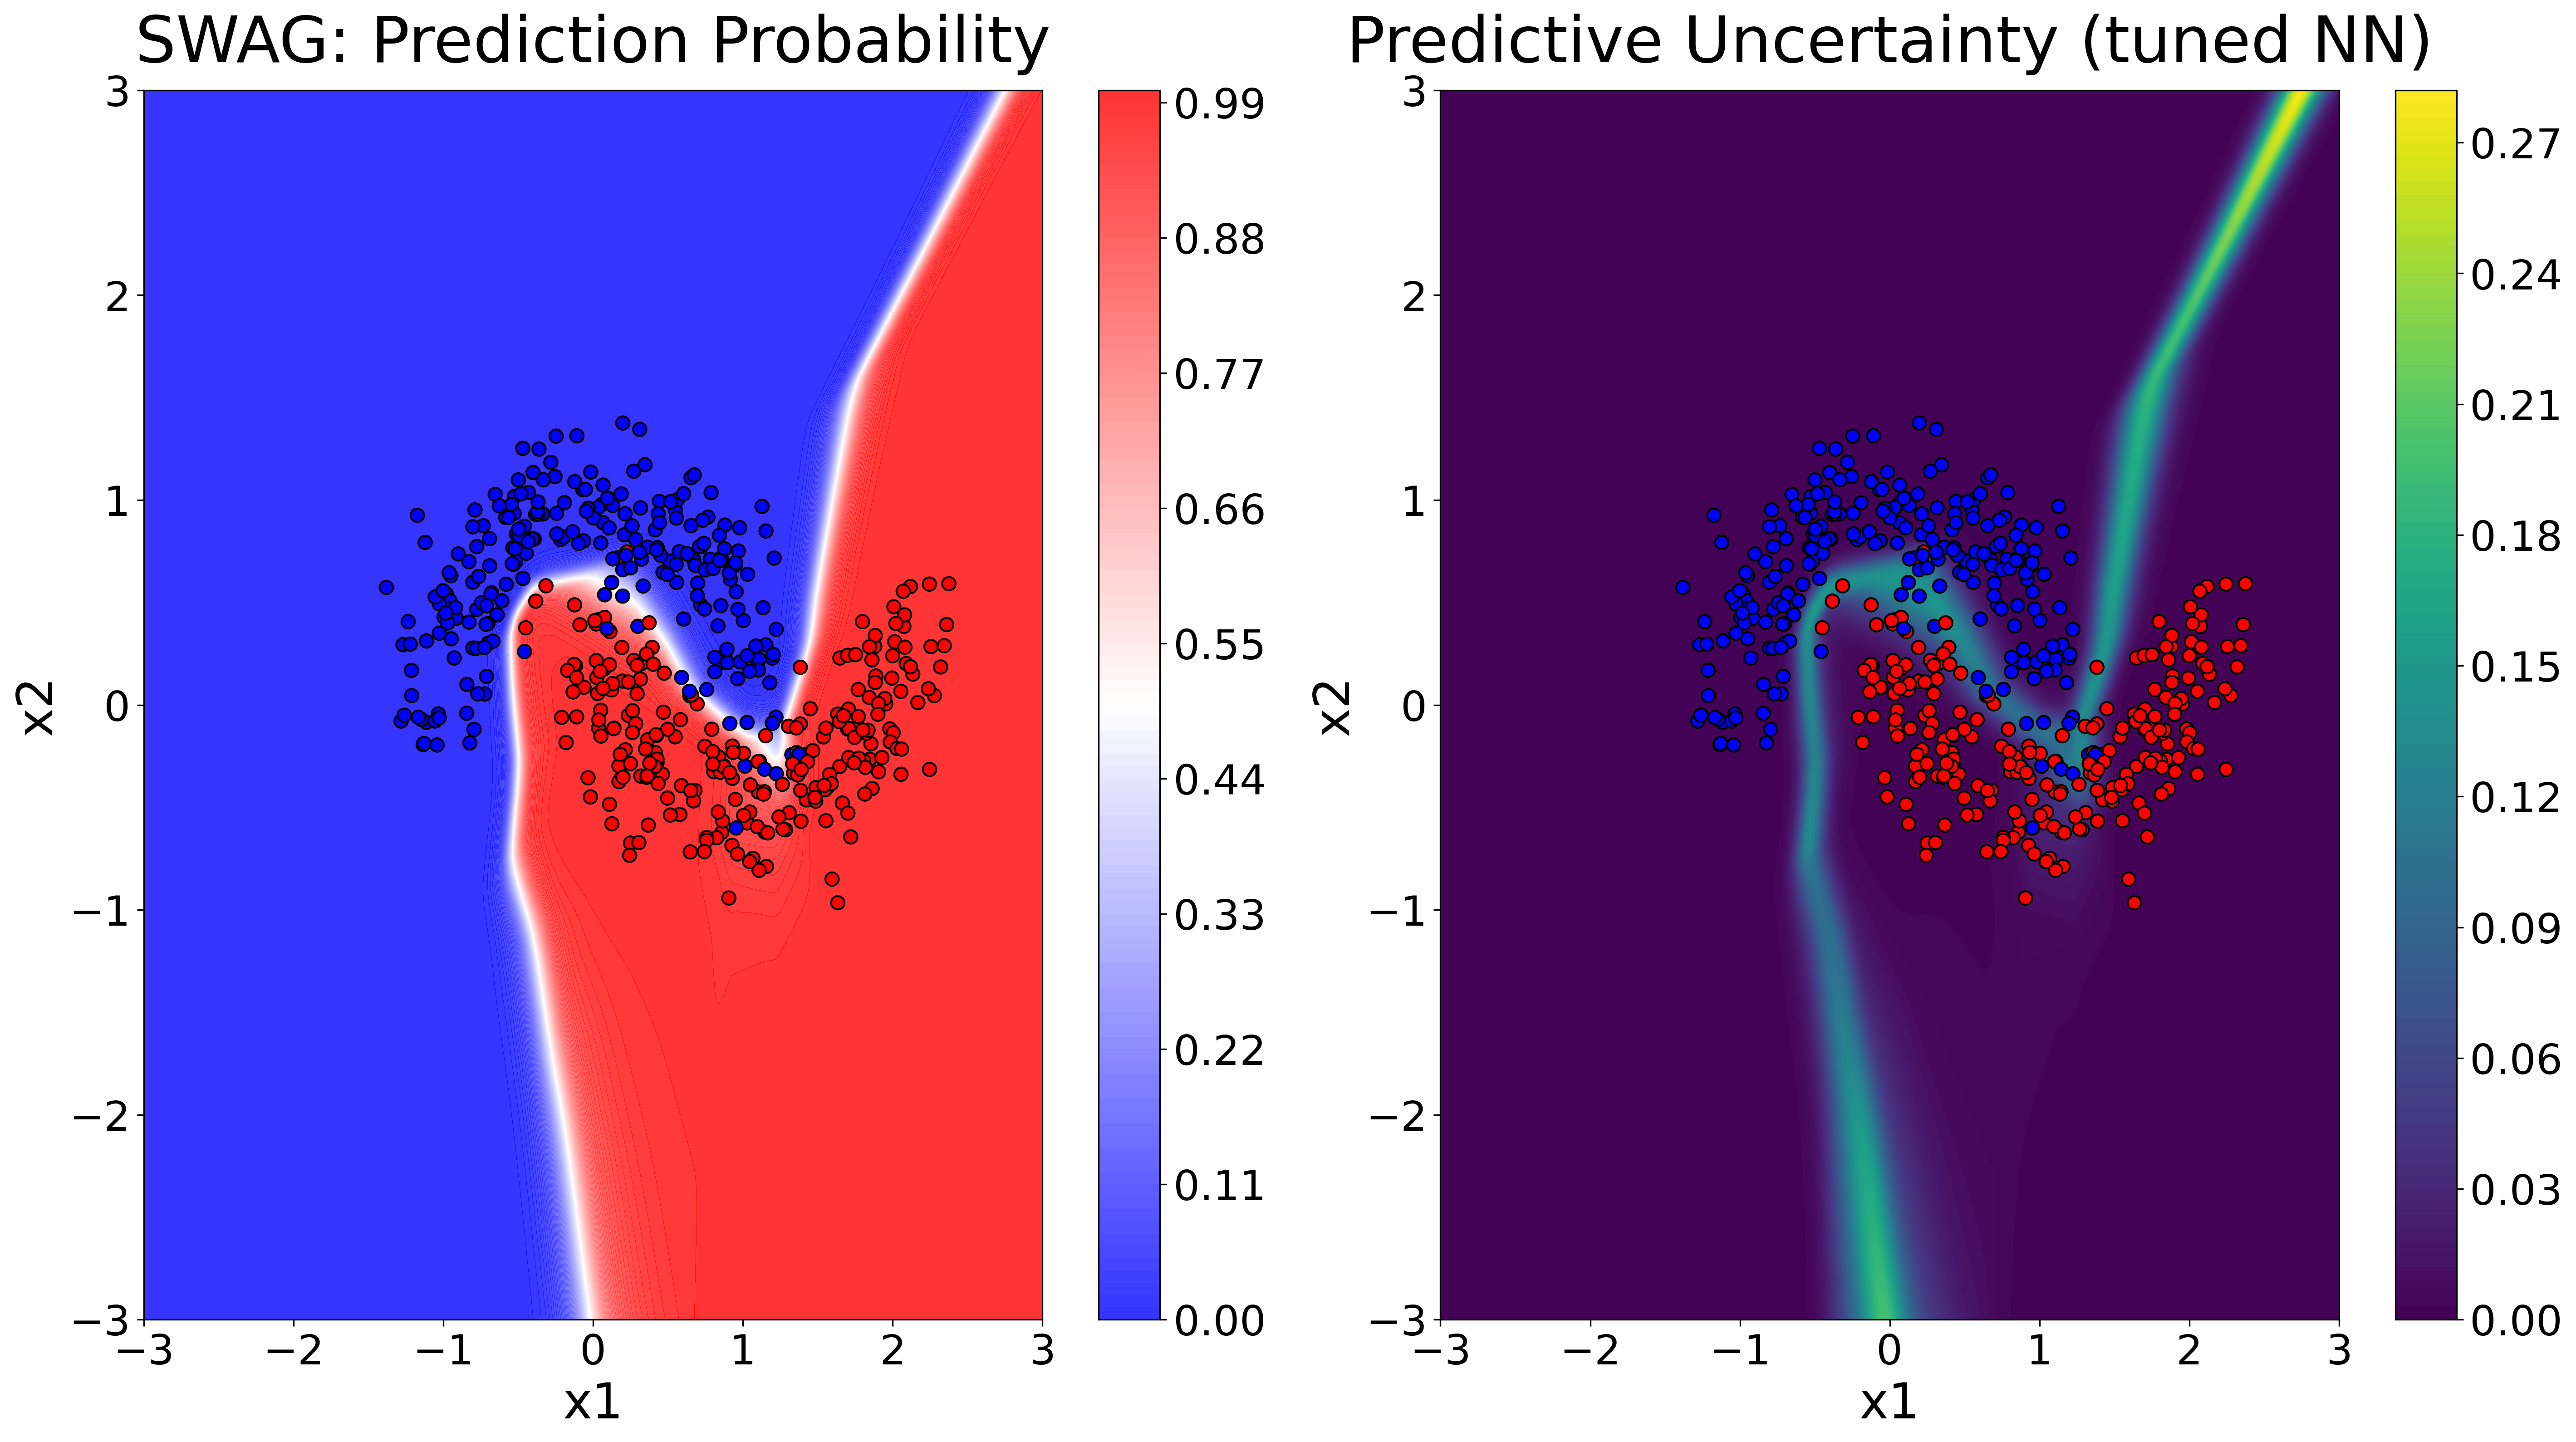
\includegraphics[width=\textwidth]{plots/swag_cla_tuned.png}
  \end{subfigure}
  \caption{Classification uncertainty of a tuned Neural Network: MC-Dropout (top) and SWAG (bottom). Color indicates true class (red/blue).}
  \label{fig:classification_tuned}
\end{figure}

\FloatBarrier

\paragraph{Effect of Dropout Rate on MC-Dropout Uncertainty}
We investigate the sensitivity of MC-Dropout uncertainty estimates to the dropout rate hyperparameter
using the synthetic regression task introduced in Section \ref{exp:synthetic}. While Figure
\ref{fig:regression} presented results with dropout rate = 0.2, we now systematically compare rates of
0.1, 0.3, 0.5 and 0.7. 

As shown in Figure \ref{fig:dropoutrate_comparison}, higher dropout rates produce progressively wider
uncertainty intervals throughout the domain, particularly in extrapolation regions ($|x| > 5$). The mean
prediction also increasingly deviates from the true function as dropout rate increases. These observations
align with findings from \citet{verdoja2021behaviormcdropout}, confirming that dropout rate selection
critically impacts both uncertainty quantification and predictive accuracy.

\FloatBarrier

\begin{figure}[ht]
    \centering
    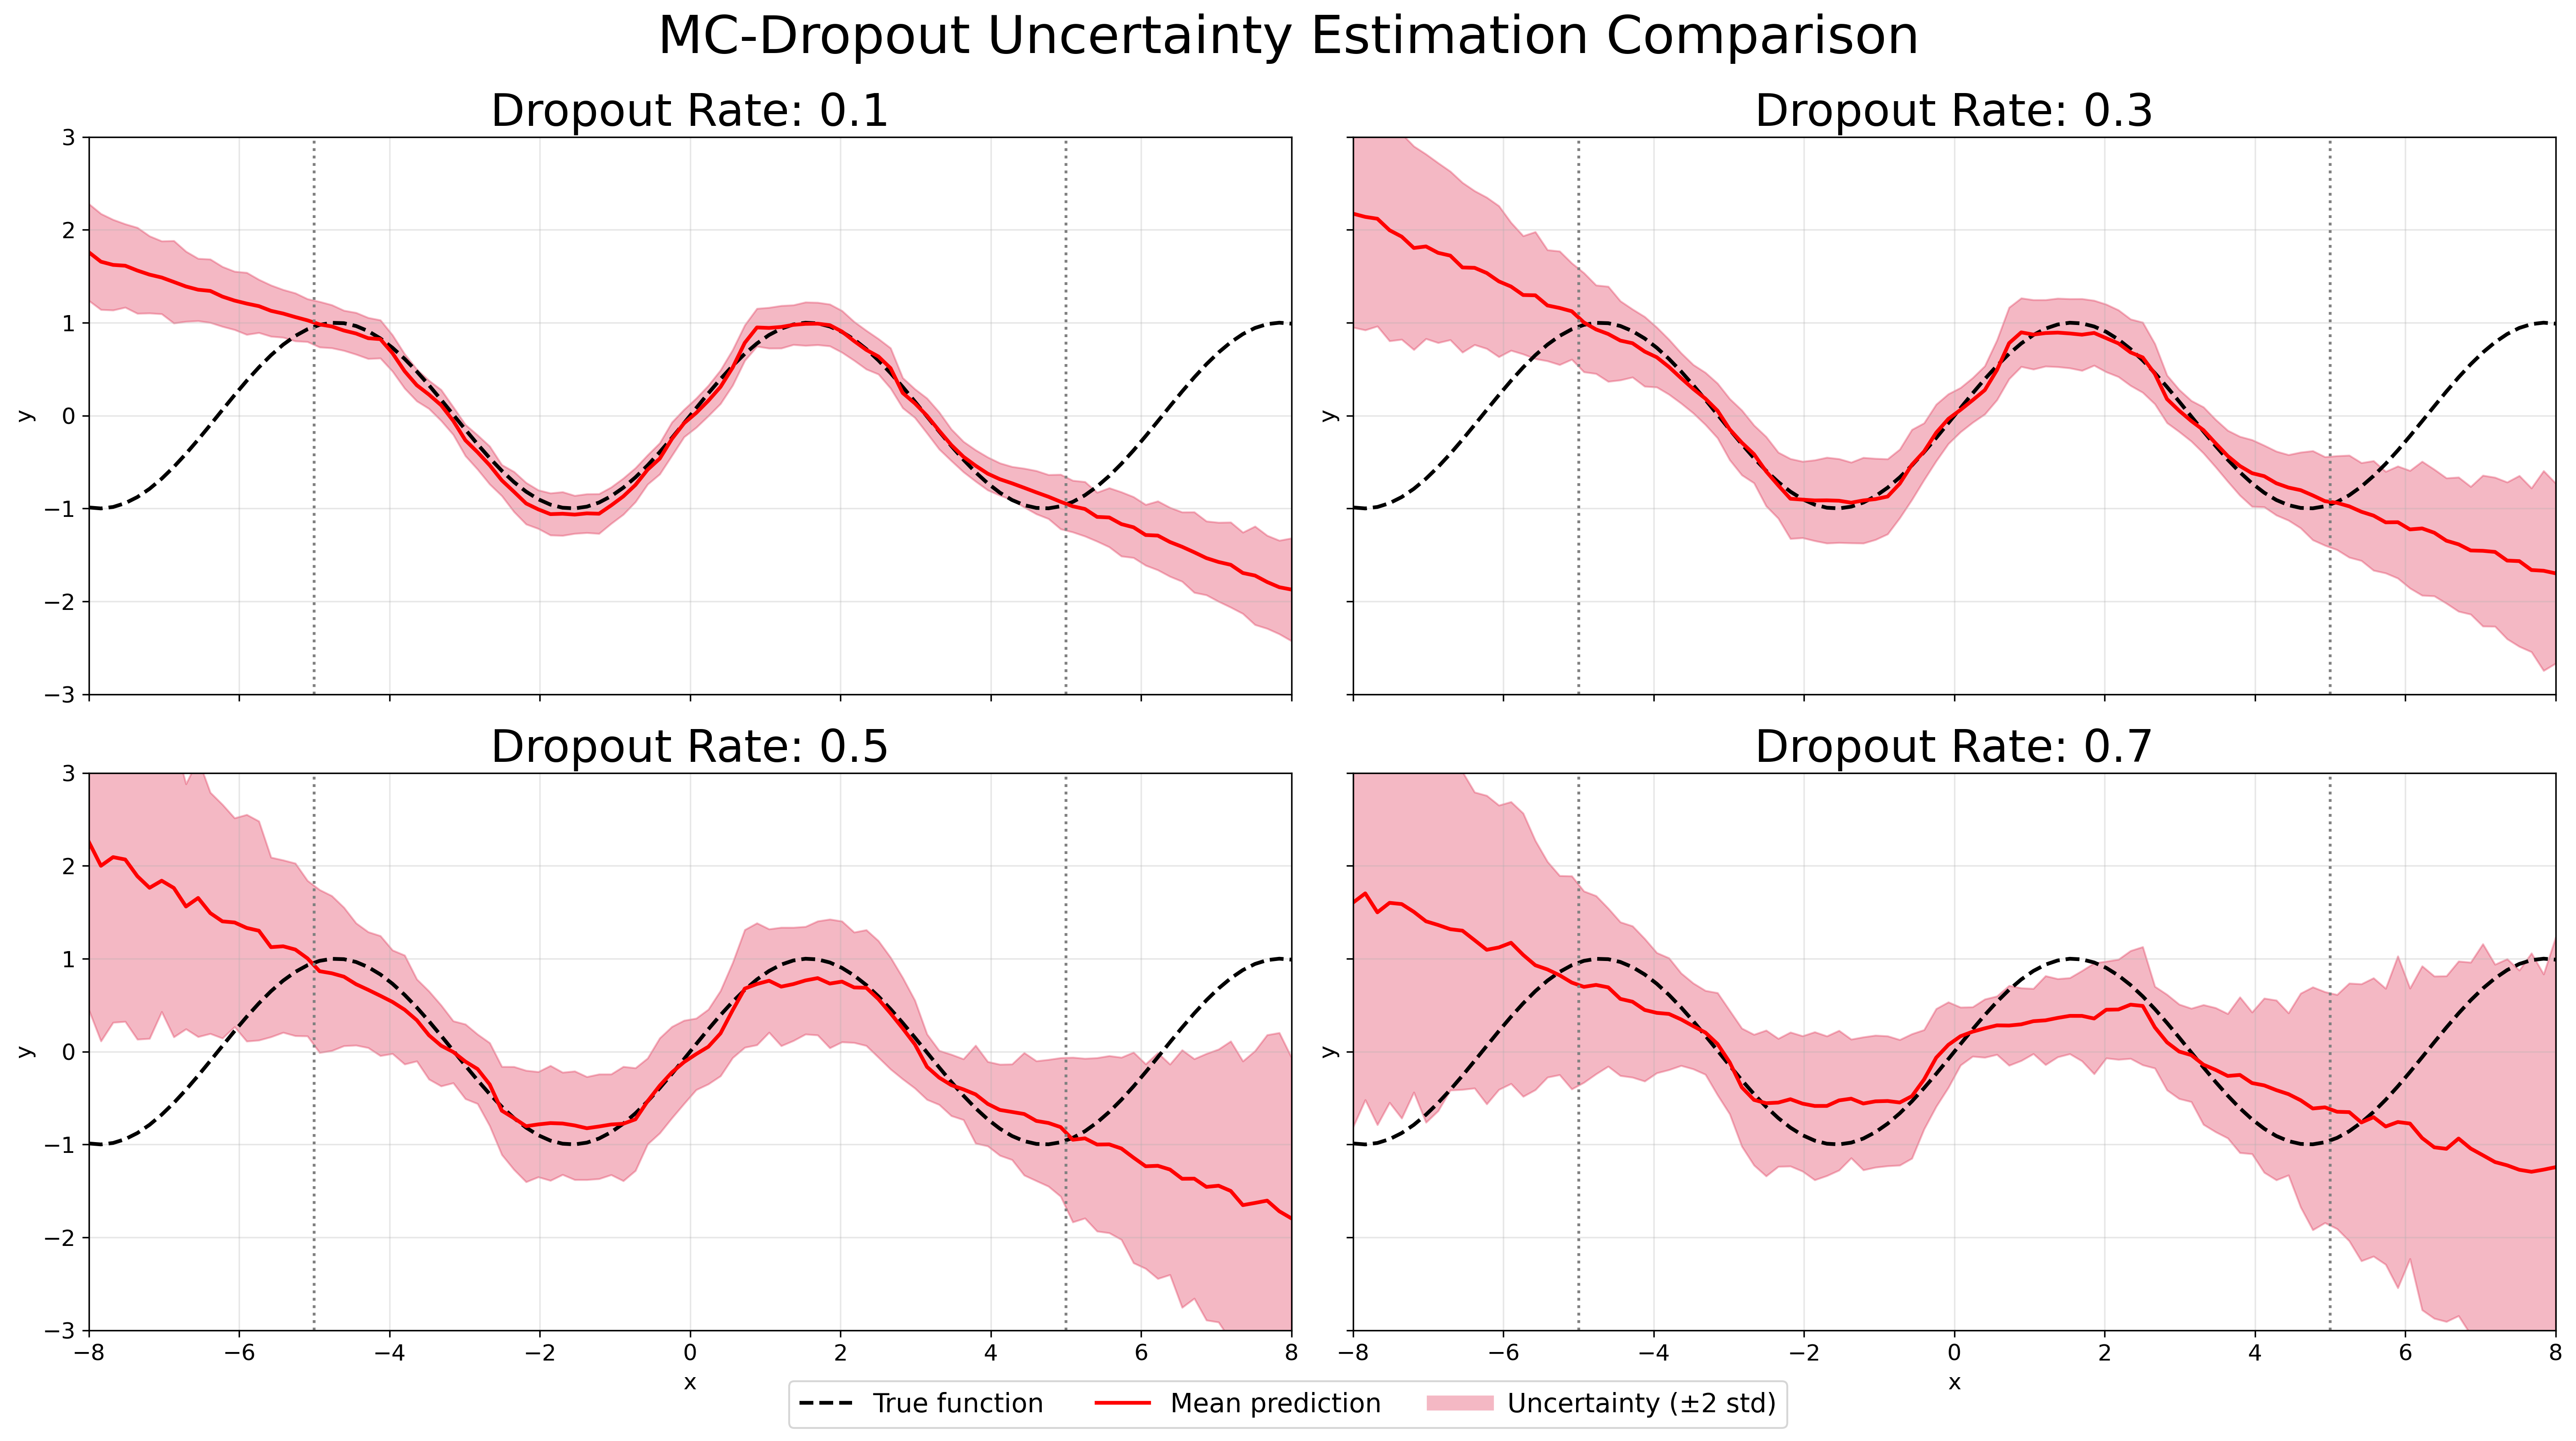
\includegraphics[width=0.9\textwidth]{plots/mcd_reg_comparison_2x2.png}
    \caption{Uncertainty estimation using MC-Dropout with different dropout rates (0.1, 0.3, 0.5, 0.7) on the same regression task.}
    \label{fig:dropoutrate_comparison}
\end{figure}

\FloatBarrier

\paragraph{Predictions with 95\,\% Confidence Intervals on Boston Housing}
Figure \ref{fig:bh_uncertainty_intervals} visualizes predictions against standardized true values with 95\,\% confidence intervals for both methods. The visualization reveals two significant patterns, SWAG exhibits consistently wider confidence intervals (orange bars), particularly pronounced for lower true values in the left side of the plot, confirming its more conservative uncertainty estimation approach. In contrast, MC-Dropout maintains narrower confidence bands that may fail to contain the true values, consistent with its undercoverage tendency. Both methods show generally accurate point predictions closely distributed around the identity line, with only two notable outliers where predictions significantly deviate from true values.

\FloatBarrier

\begin{figure}[ht]
    \centering
    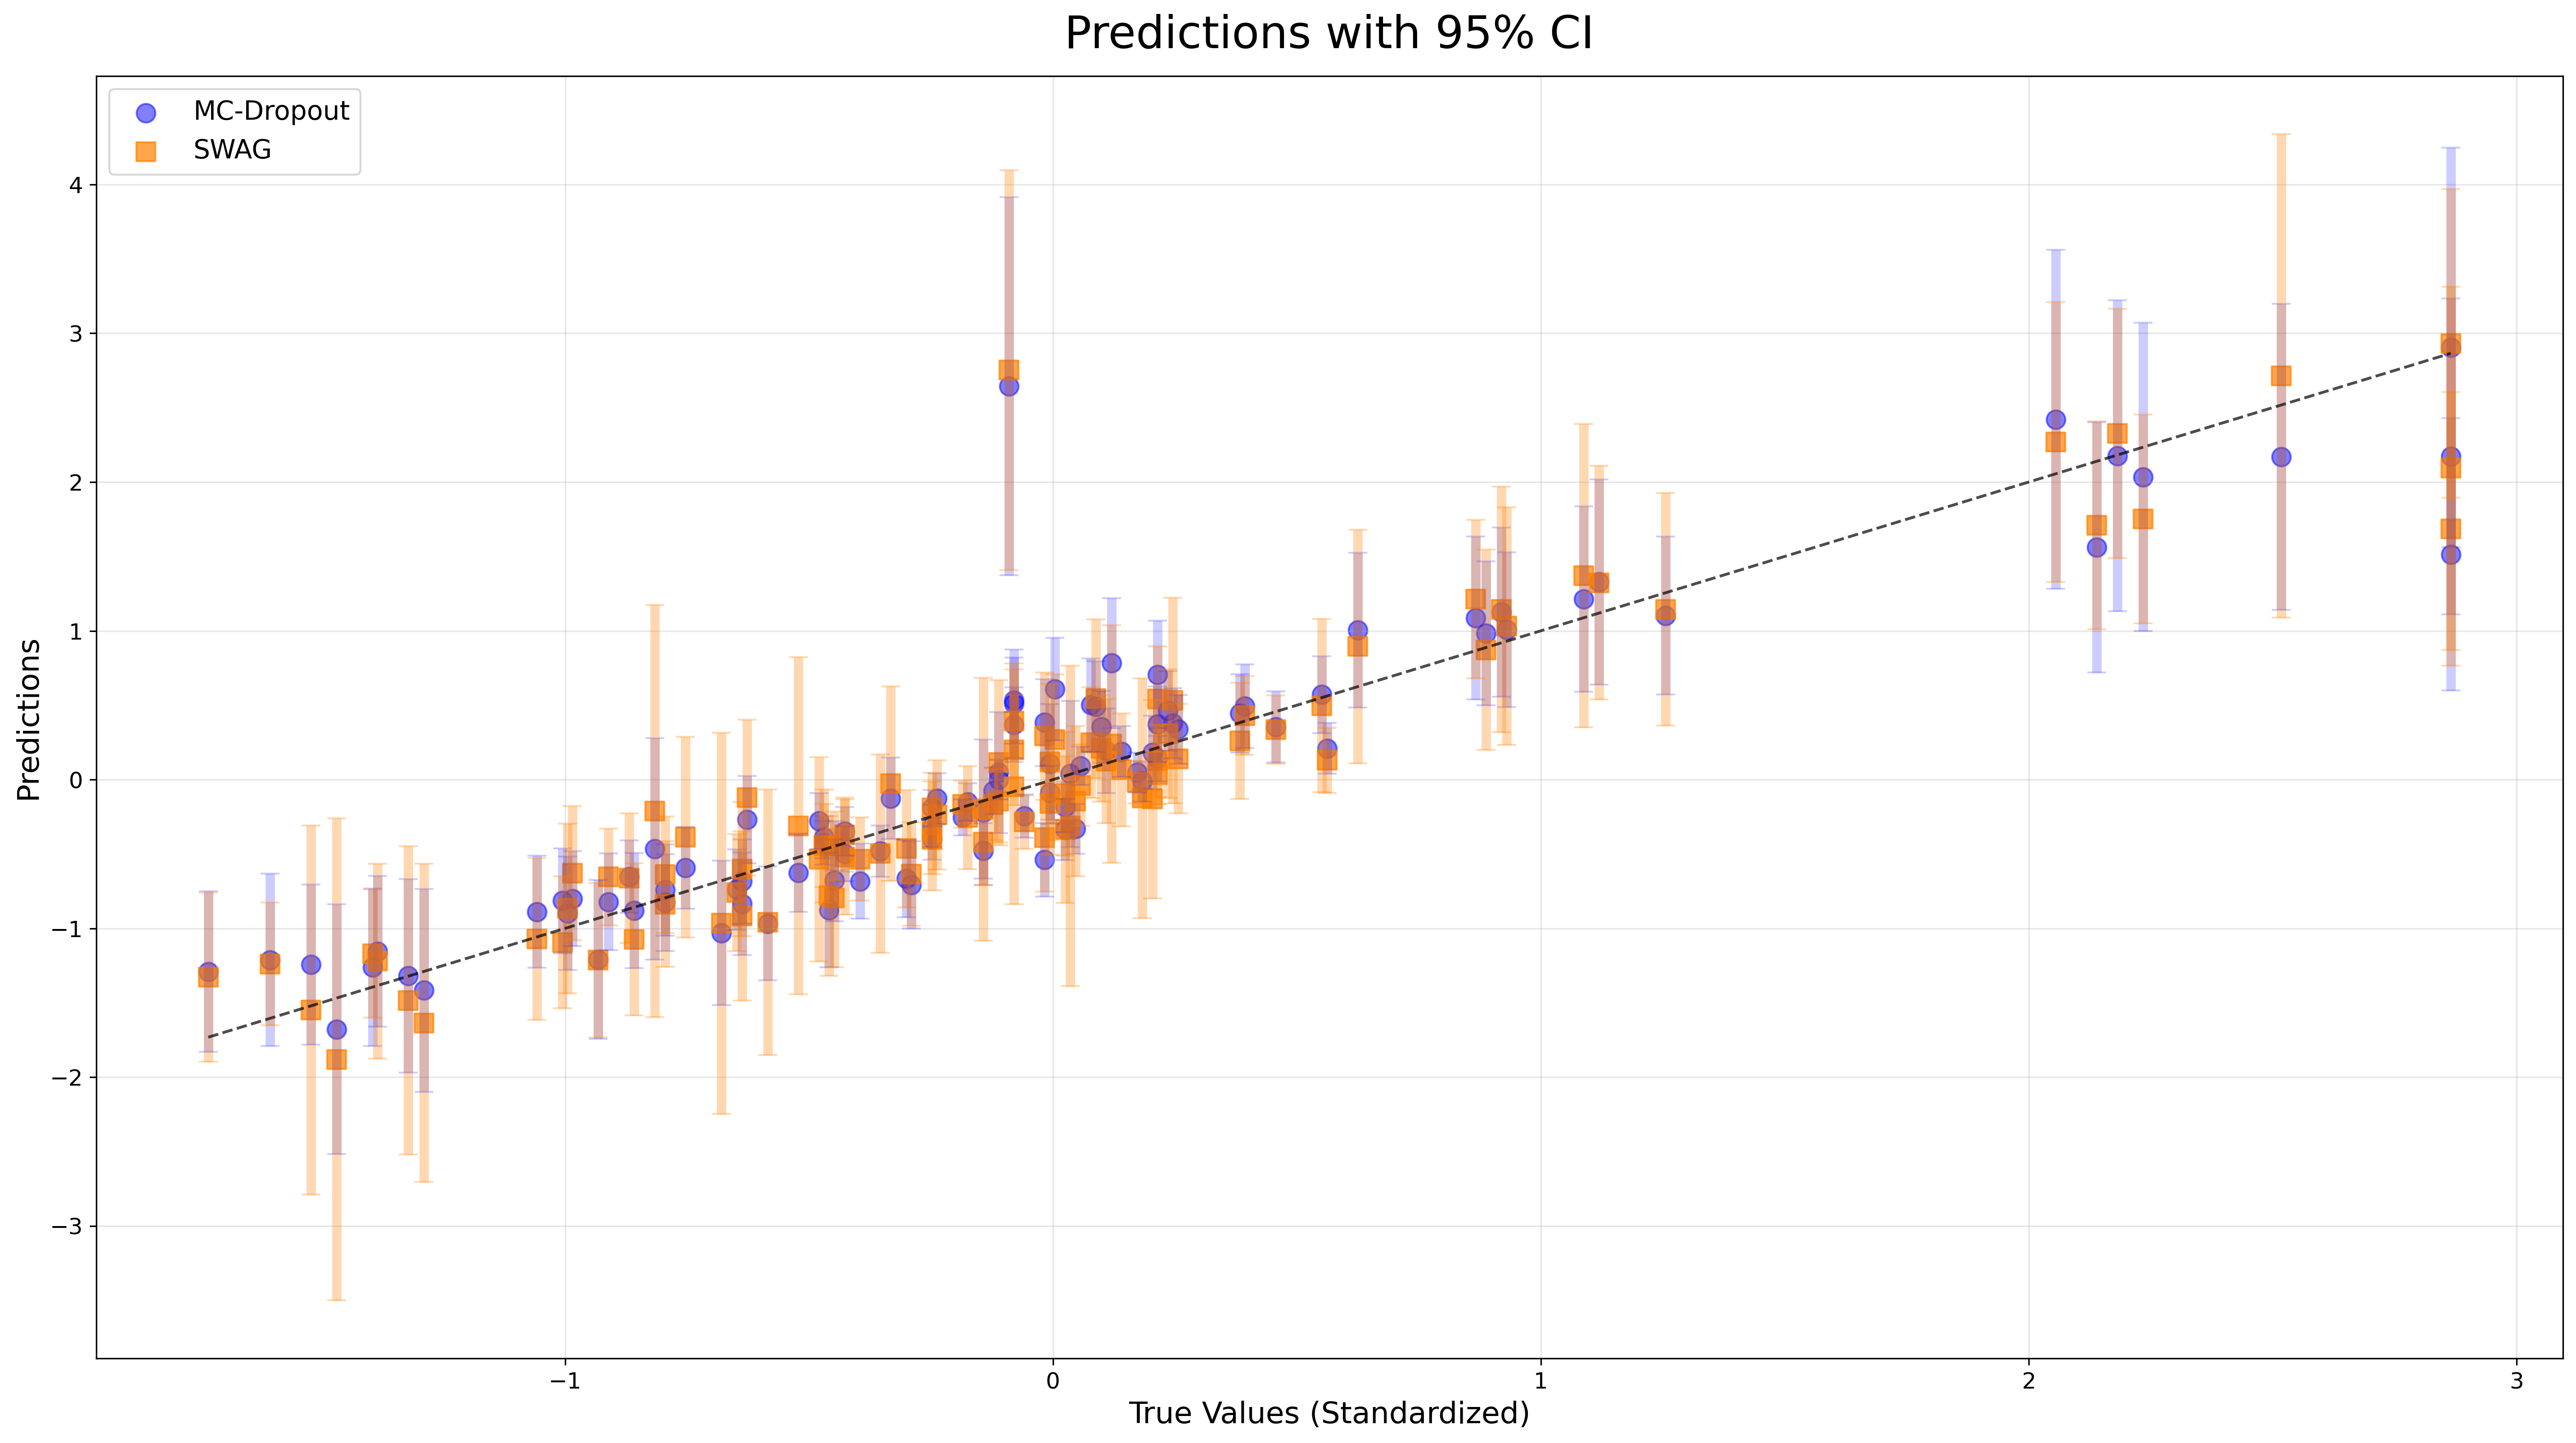
\includegraphics[width=0.9\linewidth]{plots/bh_uncertainty_intervals.png}
    \caption{Predictions with 95\,\% confidence intervals on Boston Housing test set. Dashed line represents perfect predictions (y=x).}
    \label{fig:bh_uncertainty_intervals}
\end{figure}

\FloatBarrier

\paragraph{Residual Analysis on Boston Housing}
Figure \ref{fig:bh_residuals} presents a diagnostic examination of model performance through residual analysis, where residuals represent the difference between observed and predicted values. The visualization reveals randomly distributed points for both MC-Dropout (blue) and SWAG (orange) that symmetrically scatter around the zero-reference line throughout the prediction range. Residual magnitudes demonstrate comparable dispersion for both methods, with no evidence of systematic patterns. This absence of structure indicates a well-calibrated model without significant bias or heteroskedasticity. The random error distribution confirms that both methods capture the underlying relationships in the data effectively, with prediction errors showing no directional tendency.

\FloatBarrier

\begin{figure}[htbp]
    \centering
    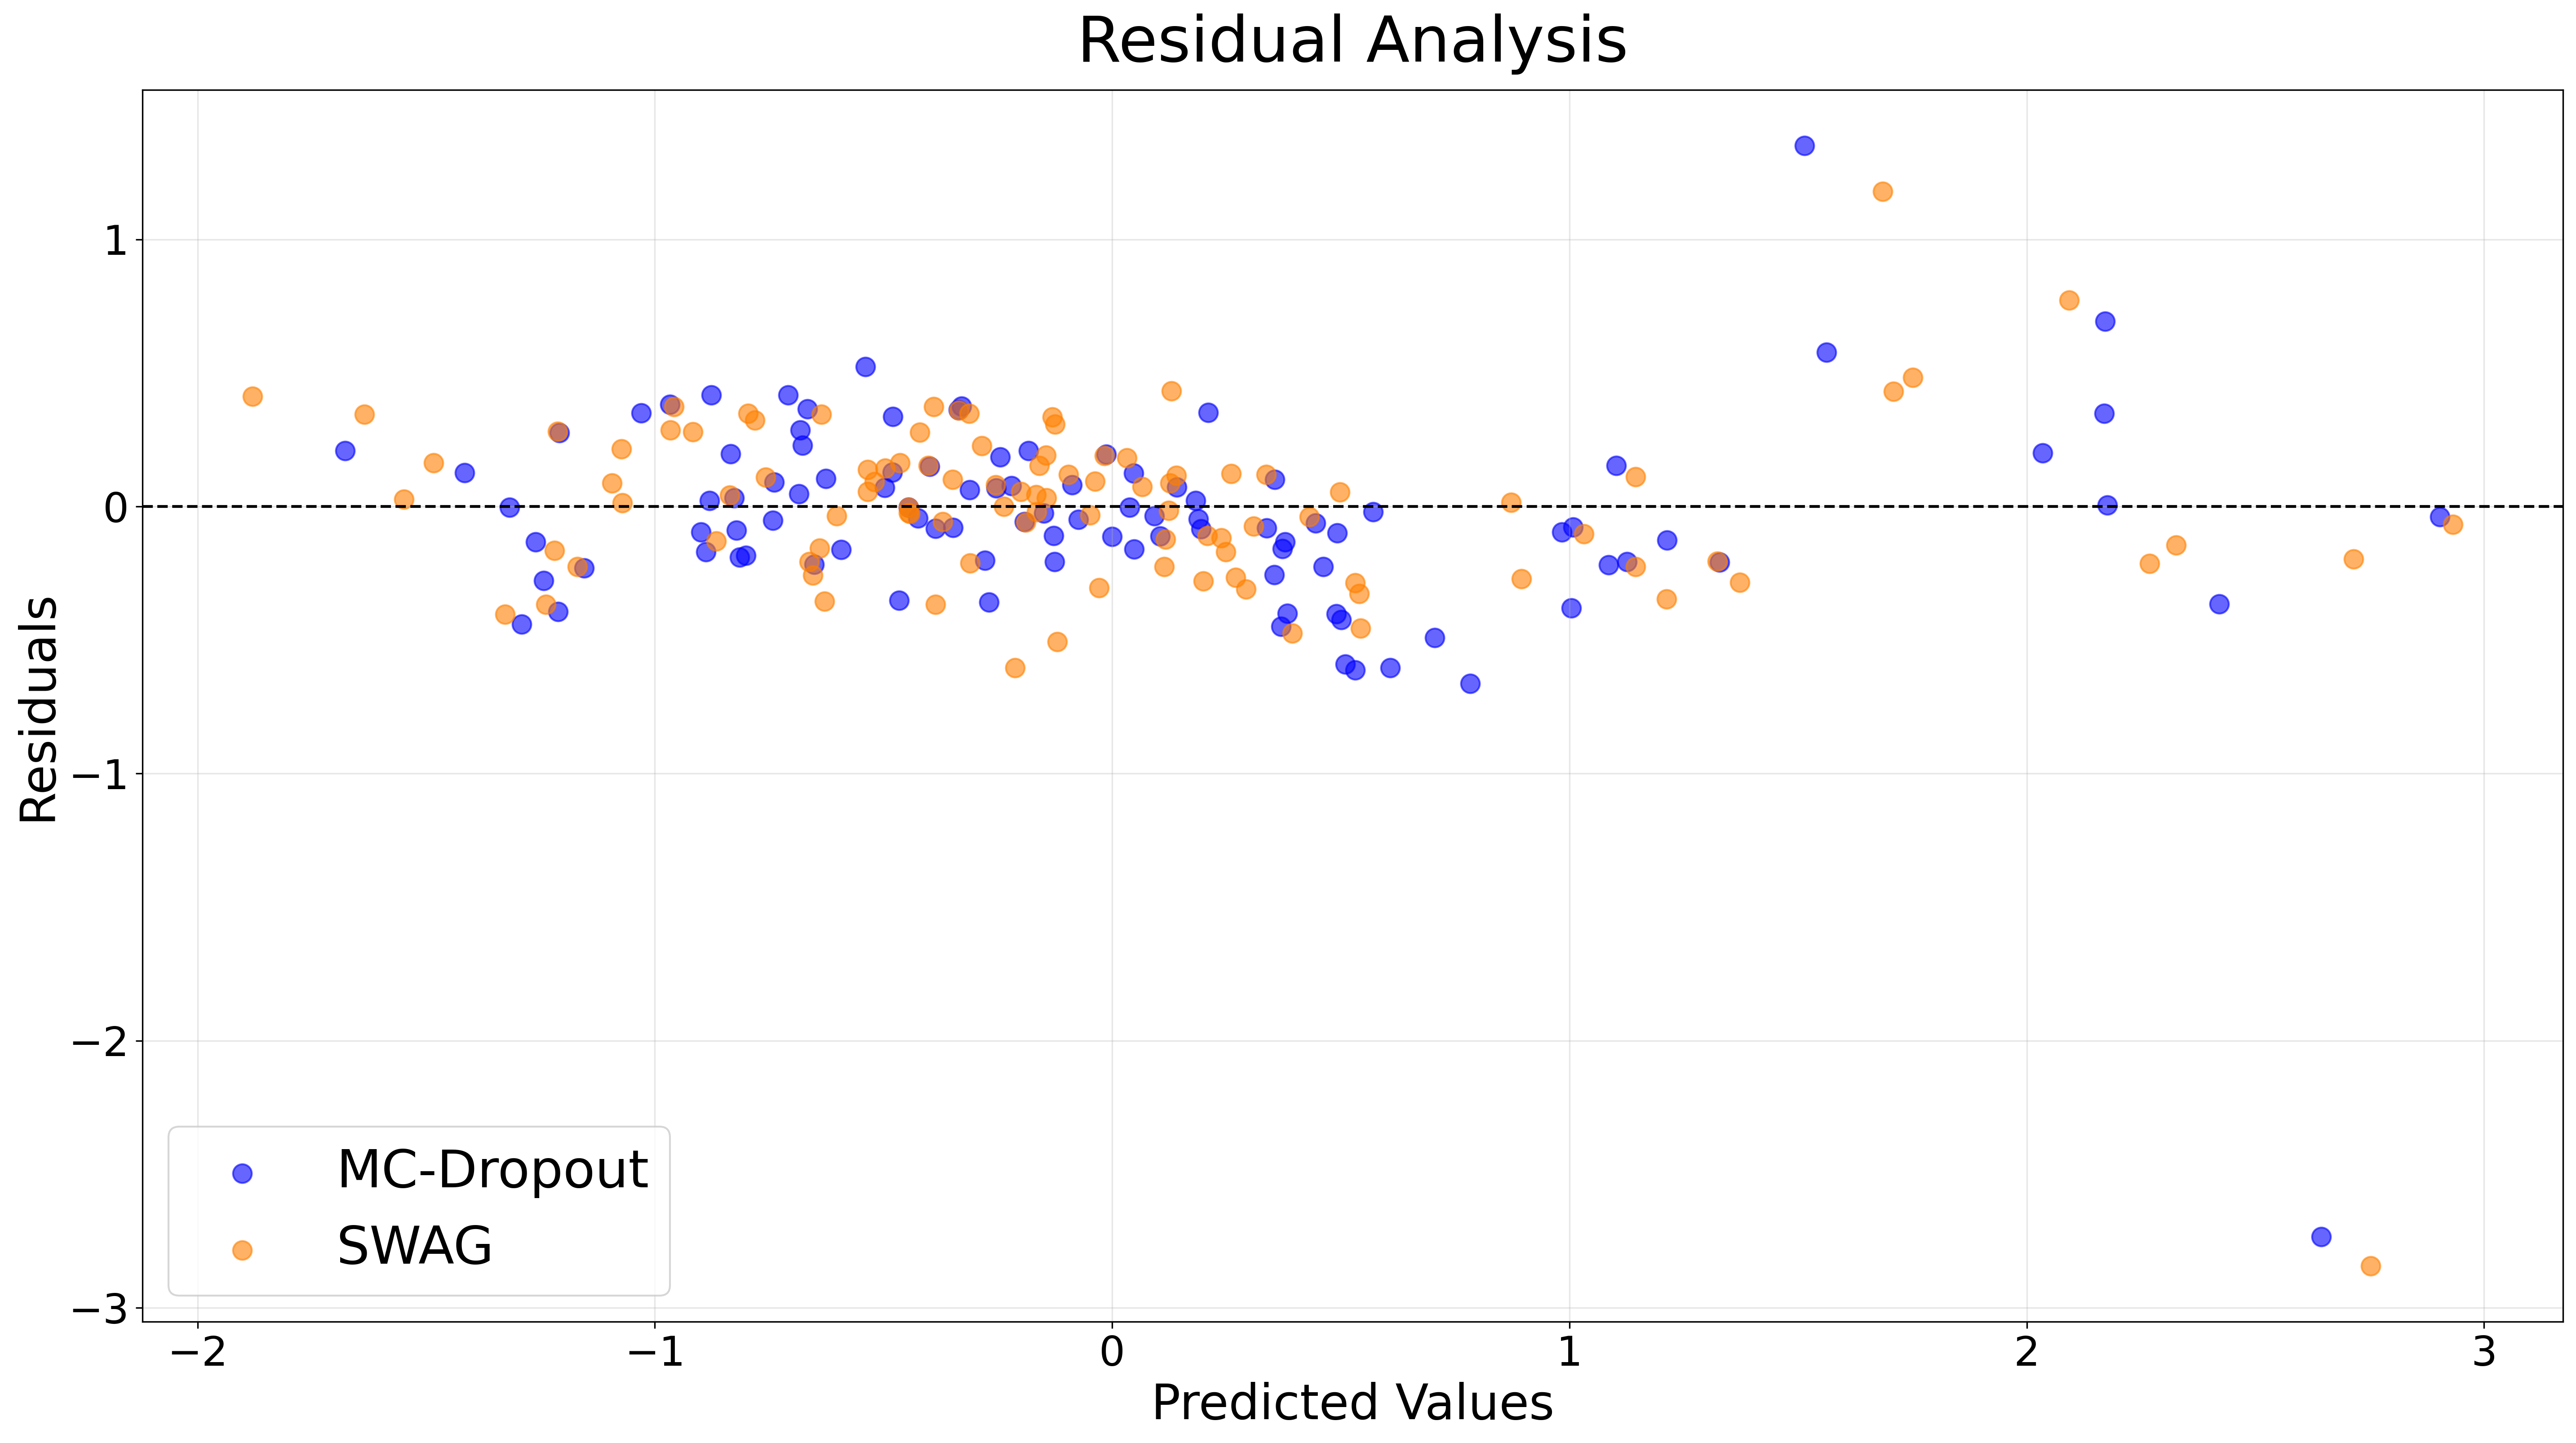
\includegraphics[width=0.9\linewidth]{plots/bh_residuals.png}
    \caption{Residual analysis for Boston Housing predictions. Dashed line represents perfect prediction (residual = 0).}
    \label{fig:bh_residuals}
\end{figure}

\FloatBarrier
